

\section{A Framework for Simulation}

The goal of simulation is the analysis of a real-world process by imitating its behaviour using computer software.
In the previous chapters we saw examples of how we could use randomness to perform calculations that are deterministic in nature (e.g. the area calculations in Section~\ref{sec2:areavolume}).
Such experiments are referred to as \textbf{Monte Carlo Methods}.

Moreover, we also performed simulations of processes for which randomness was an inherent characteristic (rolling a die, etc., in Chapter~\ref{sec3}).
Arguably this scenario is more interesting than the former, since one cannot \emph{solve} these processes analytically as one can theoretically do for area and volume calculations; outcomes of these experiments cannot be predicted (although one can derive quantities like the long-term behaviour of random processes).
And herein lies the main advantage of simulation -- it is a low-risk method for obtaining knowledge about how a random system operates (or \emph{will operate}).

In particular, \underline{what if} questions are addressed easily by simulations.
\emph{What if we change one of the starting assumptions?}
\emph{What if we remove a certain part of the system?}
These are not easy to analyze in general, but simulations may reveal what the outcomes are.

In \cite{banks2010} some commonly-used terms in simulations are defined:

\begin{itemize}
	\item \emph{system}: A group of objects that interact with each other or are interdependent, joined together to work toward a common goal.
	\item \emph{system environment}: Where the system is `located,' i.e. refers to the space outside the system but from where changes to the system can be caused.
	\item \emph{entity}: An object in the system.
	\item \emph{attribute}: A property of an entity.
	\item \emph{activity}: A time period of given length.
	\item \emph{state}: The collection of variables necessary to describe the system at any given time.
	\item \emph{event}: An instantaneous occurrence that might change the state of the system.
	\item \emph{model}: A representation of the system.
\end{itemize}

There are a few more classifications that are used to refer to systems and their simulation.

\begin{itemize}
	\item A system is \emph{discrete} if changes can only happen at a discrete set of time points, and \emph{continuous} if variables can change continuously.
	\item A simulation model is \emph{static} if it represents a system at a fixed point in time, and \emph{dynamic} if it represents a system as it changes over time.
	\item A model is called \emph{stochastic} if it contains random variables, and \emph{deterministic} otherwise.
\end{itemize}

Note that we can also refer to models as discrete or continuous, and that the type of model used may not necessarily match the type of system being observed (so a discrete model can be used to study a continuous system, and vice versa).
The term \textbf{discrete-event simulation} refers to the case when the types of models studied are discrete, dynamic, and stochastic.

Typically, simulation-based studies will follow the same framework.
First, a problem is identified and formulated.
Then, objectives are set -- what do we want to know?
Is simulation the appropriate tool?
Then a model is formulated; this may be a very involved process, and there is no single approach that will work for all problems.
In general, it is a good idea to start with a simple model, and then increase the complexity as the study moves forward.

Once the model is constructed, input data is collected, and the model programmed into a computer.
Then \emph{model verification} and \emph{model validation} are done.
This means that the model is first checked, to make sure the data representations used are appropriate, and the logic is sound (verification).
Then, the model is run on a few test cases where the real-world outcome is known, and the outputs are compared (validation).

After these steps, the actual experiment begins.
Parameters such as the maximum number of iterations, maximum time of simulation, and number of replications of each run are fixed, and input data is selected.
Then the model is run, and an analysis is carried-out on the system being studied.


\newpage

\section{Simulating Simple Queues}

Queueing is something everyone experiences in daily life -- we wait in lines at the supermarket, at the bank, when taking transit, and so on.
Routers also queue information to send to your wireless devices.
Modelling the behaviour of queues can be very involved and complicated, especially for more complex systems.
When studying a system with queues, we are interested in various properties of such as:

\begin{enumerate}[(1)]
	\item Average waiting times,
	\item Average total times in the system (including the processing time),
	\item Average size of queues,
	\item Probability of spending time in a given queue,
	\item Proportion of idle time of the server.
\end{enumerate}


To understand a queueing system, we should model arrival times for \emph{customers}, their routes through the system, and \emph{service times} once a customer is being processed.
For instance, at a supermarket we might want to analyze its queueing system for checking out.
This would involve gathering data empirically to determine what probability distribution governs the time between two customer arrivals at the queue (which may vary depending on time of day) and studying how long it takes to serve a customer.
This analysis could then be used to predict the effects of adding counters or varying the checkout procedures, e.g. through introducing express counters or self-checkout counters.

The following assumptions are typical in simple queueing models:
\begin{enumerate}[(a)]
	\item Interarrival times of the customers are drawn independently from some probability distribution $A$.
	\item Service times of successive customers are drawn independently from some probability distribution $S$.
	\item When a customer arrives and the server is idle, the customer is immediately served.
		Otherwise, if the server is busy, the customer joins the end of the queue.
\end{enumerate}

Key characteristics that differentiate one queueing system from another are the probability distributions for arrivals and service time, and the number of servers.
For now we limit our discussion to single-server queues.

\vspace{0.5cm}
\begin{figure}[htbp]
	\centering
	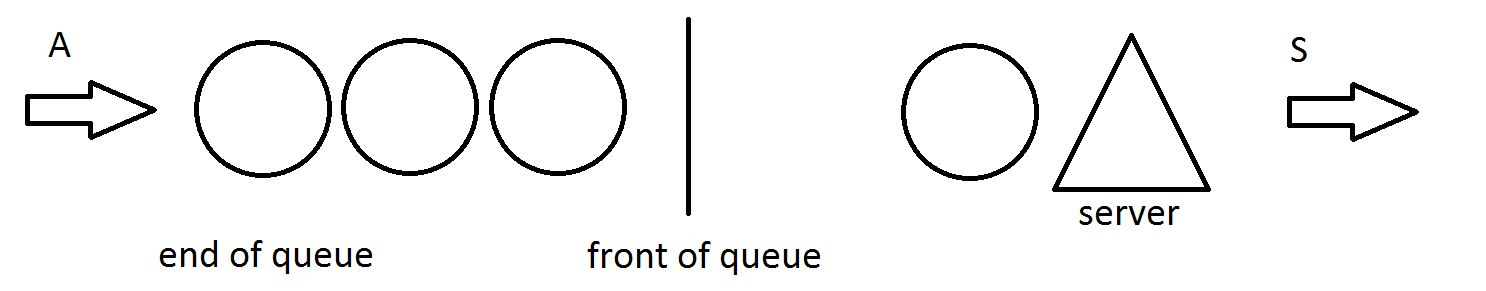
\includegraphics[width=0.9\textwidth]{fig/4_queuepaint0.png}
	\caption{A single-server queue. \label{fig:4_queuepaint0}}
\end{figure}

\vspace{0.4cm}

\newpage

\begin{myexample}\label{ex:4_queue}
	In a single-server queue, interarrival times follow the discrete uniform distribution $U\{1,6\}$.
	Customers are served in 3 minutes with probability $0.25$, 4 minutes with probability $0.5$, and 7 minutes with probability $0.25$.
	Simulate this process until 10 customers are served, and find the average waiting time of a customer.

First, we have to generate interarrival times. 
Suppose that we used Excel to do this, and obtained the following: 4, 3, 5, 5, 5, 1, 4, 2, 5, 3 (using the \texttt{=RANDBETWEEN()} function).

Next, we generate service times, and obtain: 4, 7, 4, 3, 3, 3, 4, 7, 4, 4 (using the \texttt{IF()} function with \texttt{RAND()}).

Assuming we start at time $t = 0$, the first customer arrives at time $t = 4$.
Since the server is idle when he arrives, he is served immediately. 


\begin{figure}[htbp]
	\centering
	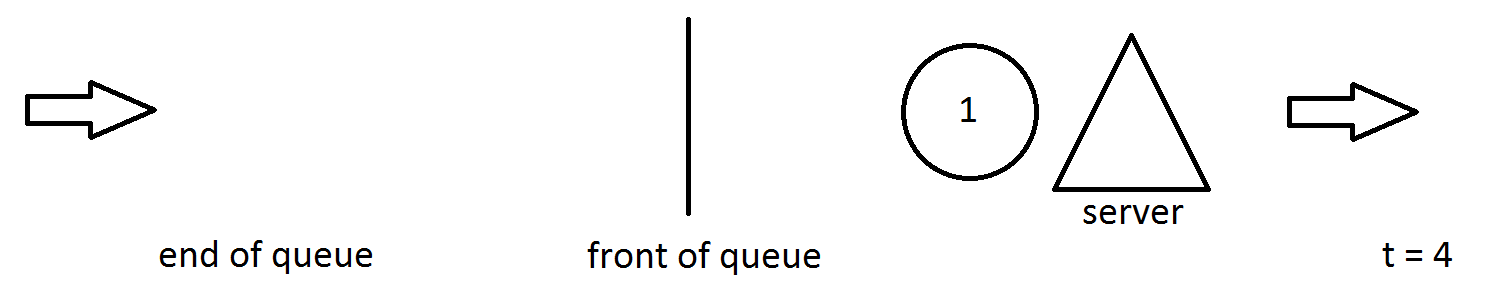
\includegraphics[width=0.8\textwidth]{fig/4_queue_ex1a.png}
	\caption{State of the system at $t = 4$. \label{fig:4_queue_ex1a}}
\end{figure}

The service time for the first customer is 4 minutes.
Before he finishes being served, however, the second customer arrives at time $t = 4 + 3 = 7$.


\begin{figure}[htbp]
	\centering
	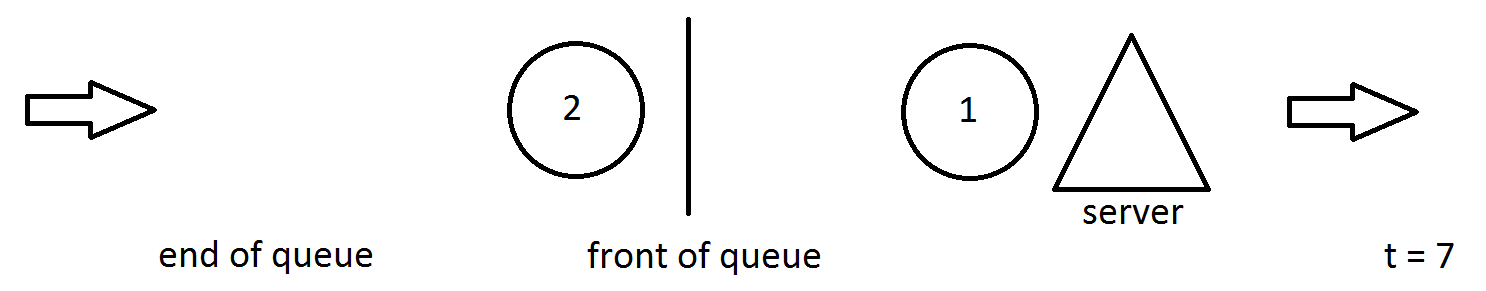
\includegraphics[width=0.8\textwidth]{fig/4_queue_ex1b.png}
	\caption{State of the system at $t = 7$. \label{fig:4_queue_ex1b}}
\end{figure}


The first customer exits the system at $t = 8$, at which point the second customer is served, with service time $7$ minutes.
The third customer arrives at time $t = 12$, and has to wait in the queue for 3 minutes until the second customer exits.

\begin{figure}[htbp]
	\centering
	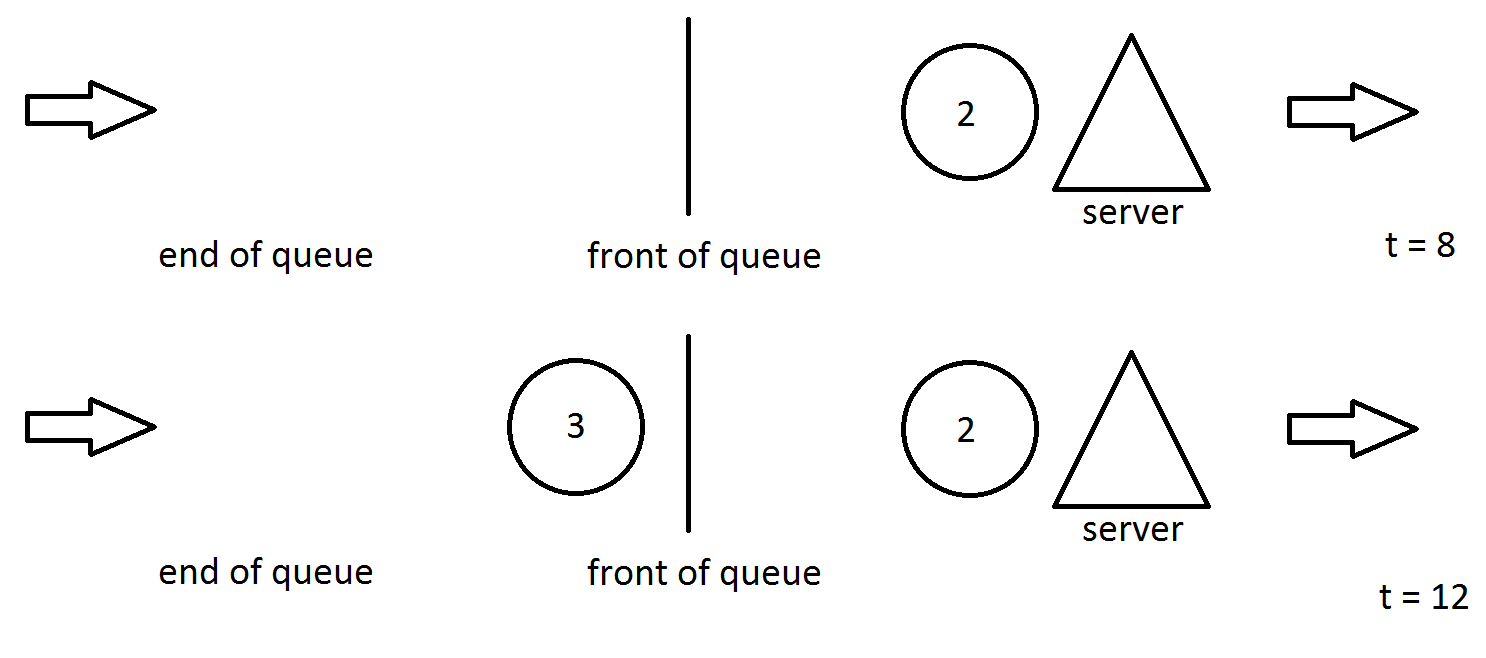
\includegraphics[width=0.8\textwidth]{fig/4_queue_ex1c.png}
	\caption{States of the system at $t = 8$ and $t = 12$. \label{fig:4_queue_ex1c}}
\end{figure}

The rest of the system behaviour can be derived similarly.
Putting everything in a table, we obtain the following values.
The waiting time of a customer is the time between arrival time and when service begins, while the total time in the system is the sum of the waiting time and the service time.

{\small
\begin{center}
\begin{tabular}{cccccccc}
	\multirow{2}{*}{Customer} & Interarrival & Time of & Service & Service & Service & Waiting & Total time \\
	& times & arrival & time & start & end & time & in system \\
\hline
1 & 4 & 4 & 4 & 4 & 8 & 0 & 4 \\
2 & 3 & 7 & 7 & 8 & 15 & 1 & 8 \\
3 & 5 & 12 & 4 & 15 & 19 & 3 & 7 \\
4 & 5 & 17 & 3 & 19 & 22 & 2 & 5 \\
5 & 5 & 22 & 3 & 22 & 25 & 0 & 3 \\
6 & 1 & 23 & 3 & 25 & 28 & 2 & 5 \\
7 & 4 & 27 & 4 & 28 & 32 & 1 & 5 \\
8 & 2 & 29 & 7 & 32 & 39 & 3 & 10 \\
9 & 5 & 34 & 4 & 39 & 43 & 5 & 9 \\
10 & 3 & 37 & 4 & 43 & 47 & 6 & 10
\end{tabular}
\end{center}
}

The average waiting time of a customer in this system is therefore 2.3 minutes, while the average time a customer spends in the system is 6.6 minutes.
Certainly, the table can (and should) be calculated using Excel.
The long-run averages can be computed analytically -- however in this example, in the long run the queue will grow as the average service time is longer than the average interarrival time, meaning the long-run wait times diverge to infinity.
However this behaviour may not be apparent when simulating only a limited number of customers in Excel. \qed


\end{myexample}

In general, queues are represented using the notation A/S/$n$, where A represents the arrival time distribution, S the service time distribution, and $n$ the number of servers.

When interarrival times and service times are both exponentially distributed, we call the queue an M/M/$n$ queue (where `M' stands for \emph{memoryless} or \emph{Markov}).
This is one of the simplest types of queue to analyze, and provides a convenient model for many applications.
Conventionally, the parameters for these distributions are called $\lambda$ and $\mu$ (so interarrival times are Exp($\lambda$) and service times are Exp($\mu$)).


The queue in Example~\ref{ex:4_queue} can be referred to as a G/G/1 queue, where G stands for general probability distribution -- that is, it is not one of the common ones encountered.
\footnote{See the wiki page \url{https://en.wikipedia.org/wiki/Kendall's\_notation}.}

\iffalse
\begin{figure}[htbp]
	\centering
	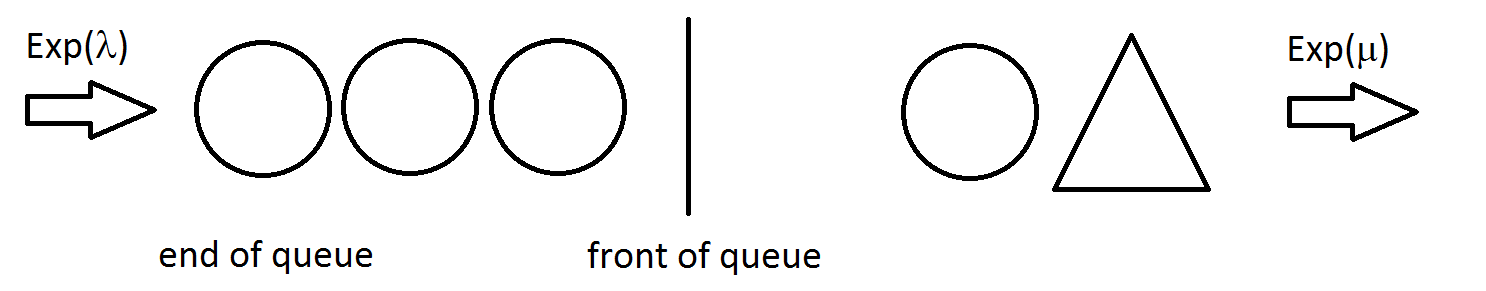
\includegraphics[width=0.8\textwidth]{fig/4_queuepaint.png}
	\caption{An M/M/1 queue. \label{fig:4_queuepaint}}
\end{figure}
\fi

\begin{figure}[htbp]
	\centering
	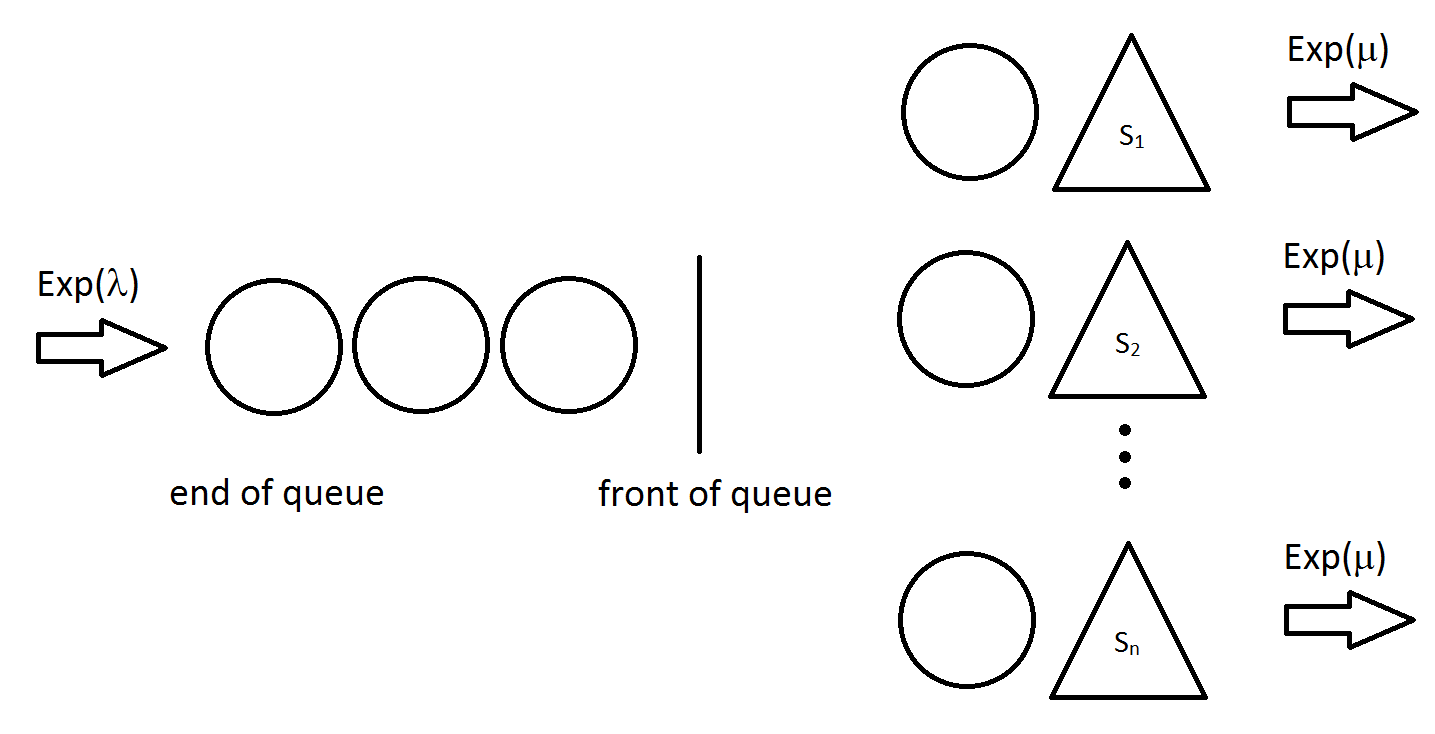
\includegraphics[width=0.6\textwidth]{fig/4_queuepaintMMn.png}
	\caption{An M/M/$n$ queue. \label{fig:4_queuepaintMMn}}
\end{figure}


\begin{myexample}\label{ex:4_MM1}
	Suppose that a queue follows the M/M/1 model with interarrival times distributed as Exp($3$) and service times distributed as Exp($5$), where a unit of time is 1 hour.
	This means that on average, 3 customers arrive in an hour, and the server can serve 5 customers in an hour,
 i.e.~$\lambda=3$ and $\mu=5$.
	Simulate this queue for 20 customers and compute the average waiting time and the average total time in the system for a customer.


To simulate this in Excel, we need to generate two sequences of values from Exp($\lambda$) and Exp($\mu$), and use these values to calculate waiting times and other statistics about the system.
Recall that we use the formula $-\frac{\ln(1-\texttt{RAND()})}{\lambda}$ to sample from Exp($\lambda$).
The spreadsheet in Figure~\ref{fig:4_queue1} shows an Excel simulation for 20 customers given $\lambda = 3$/hour and $\mu = 5$/hour.
Observe that the time a customer starts to be served depends on both the arrival time and the service end time of the previous customer, hence in cell \texttt{D6} we have the formula \texttt{=MAX(C6,E5)}.
Also note that we multiply the randomly-generated times by 60 to express them in minutes.
The waiting time being 0 means that when the customer arrives the server is immediately available.

\vspace{0.5cm}

\begin{figure}[htbp]
	\centering
	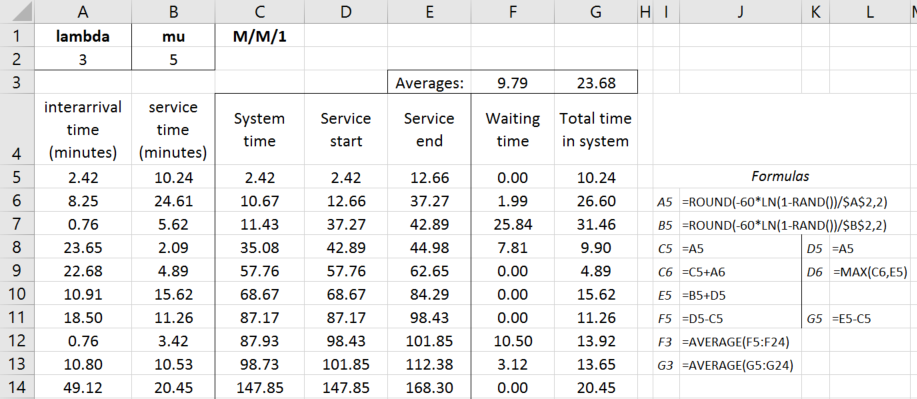
\includegraphics[width=\textwidth]{fig/4_queue1.png}
	\caption{Simulating an M/M/1 queue in Excel. \label{fig:4_queue1}}
\end{figure}

In order to calculate the statistics we are interested in, we take the average of the entries for waiting times and total time in system.
The spreadsheet allows for varying the parameters $\lambda$ and $\mu$, so that the queueing system can be studied effectively for different cases.
For instance, if customers arrive faster than they can be served ($\lambda > \mu$), the system intuitively would not be able to keep up, and the total time a customer spends in the system grows exponentially as more arrive.

To produce a visual representation for this simulation, we input the arrival time, waiting time, and service time for each customer in three columns, and use the \emph{stacked bar} chart in Excel.
Changing the fill of the first series to `no fill' will produce the following, where the red bars denote waiting times, and green denotes service times.
\footnote{This follows the method described in \cite{ig2002}.} \qed


\begin{figure}[htbp]
	\centering
	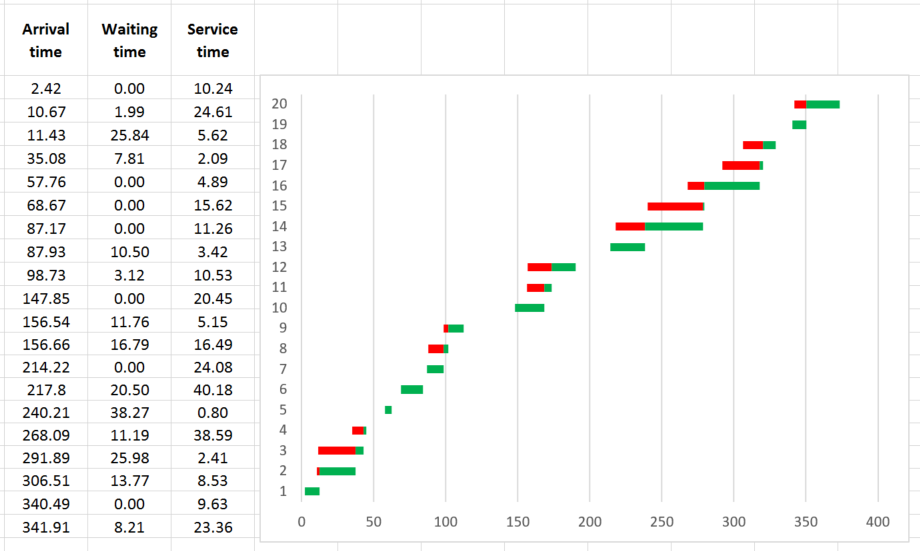
\includegraphics[width=0.95\textwidth]{fig/4_queue1chart.png}
	\caption{Visualizing an M/M/1 queue in Excel. \label{fig:4_queue1chart}}
\end{figure}

\end{myexample}

The M/M/1 queue is the simplest model to analyze; given interarrival time and service time distributions of Exp($\lambda$) and Exp($\mu$) respectively, the following quantities can be derived for the case $\lambda < \mu$:

\begin{itemize}
	\item Utilization rate is $\rho$, which is defined to be $\rho = \lambda/\mu$
	\item Average waiting time is $\frac{\rho}{\mu(1-\rho)}$
	\item Average total time in system is $\frac{1}{\mu(1 - \rho)}$
	\item Average number of customers in the system at any given time is $\frac{\rho}{1-\rho}$
\end{itemize}

If $\lambda \leq \mu$, the queue grows indefinitely since the server cannot keep up with the number of arriving customers.

Similar quantities can be derived for the more general M/M/$n$ case.
These models are more difficult to simulate in Excel -- for instance, when simulating an M/M/2 queue, for each arrival there are now three cases: server \#1 is available, server \#2 is available (but not \#1), or neither is available.

In Figure~\ref{fig:4_queue2} we show a spreadsheet simulation for the M/M/2 queue, where interarrival times are Exp($\lambda$) and service times are Exp($\mu$) for both servers, with $\lambda = 5$/hour and $\mu = 4$/hour.
Note that cells in columns \texttt{E} and \texttt{H} keep track of the earliest time each server will be available for that customer.
A graph similar to the M/M/1 case can also be generated here, by taking the same three series: arrival time, waiting time, and service time.

\begin{figure}[htbp]
	\centering
	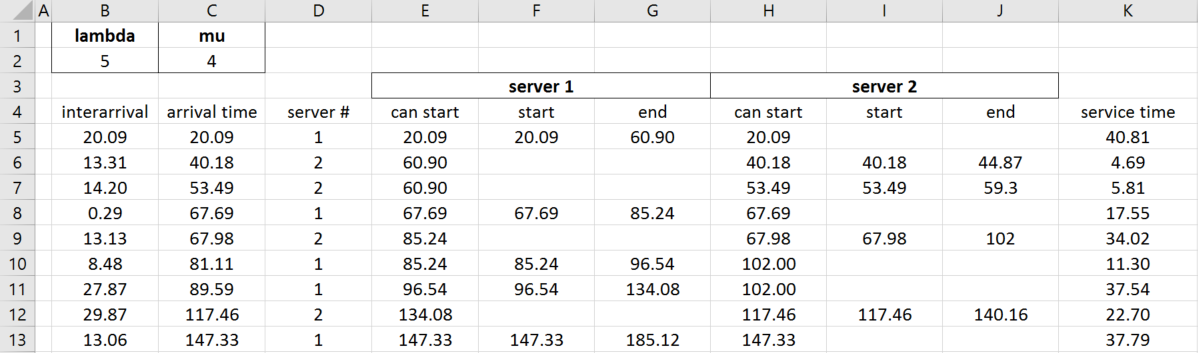
\includegraphics[width=0.95\textwidth]{fig/4_queue2.png}
	\caption{Simulating an M/M/2 queue in Excel -- times are in minutes. \label{fig:4_queue2}}
\end{figure}

\begin{figure}[htbp]
	\centering
	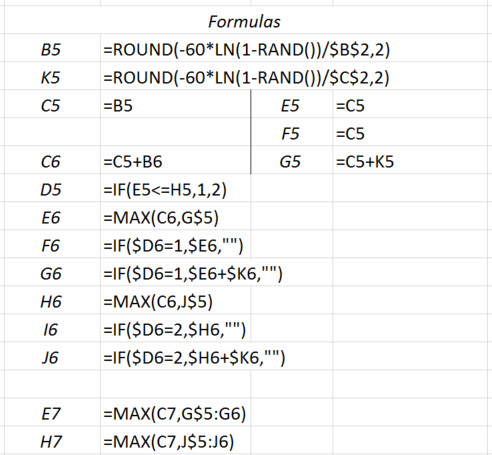
\includegraphics[width=0.4\textwidth]{fig/4_queue2formulas.png}
	\caption{Excel formulas for simulating an M/M/2 queue. \label{fig:4_queue2formulas}}
\end{figure}

\begin{figure}[htbp]
	\centering
	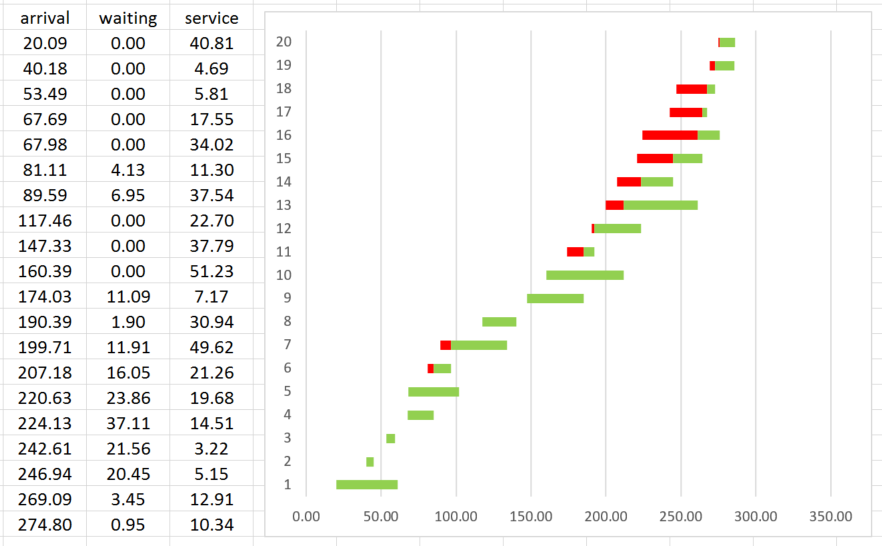
\includegraphics[width=0.8\textwidth]{fig/4_queue2chart.png}
	\caption{Visualizing an M/M/2 queue in Excel. \label{fig:4_queue2chart}}
\end{figure}

\newpage

\section{Simulating Real-time Games}

Here we consider a more detailed simulation of a real-time system: modeling a hockey game.
In hockey, teams of skaters score goals by shooting a puck into their opponent's net.
It is played between two teams of six: this includes the goaltender and five other players who are trying to score.
The game is composed of three 20-minute periods, the team with more goals at the end wins. 
Ties are broken in varying ways depending on the type of game played (professional/amateur, regular/playoff).

\begin{figure}[htbp]
	\centering
	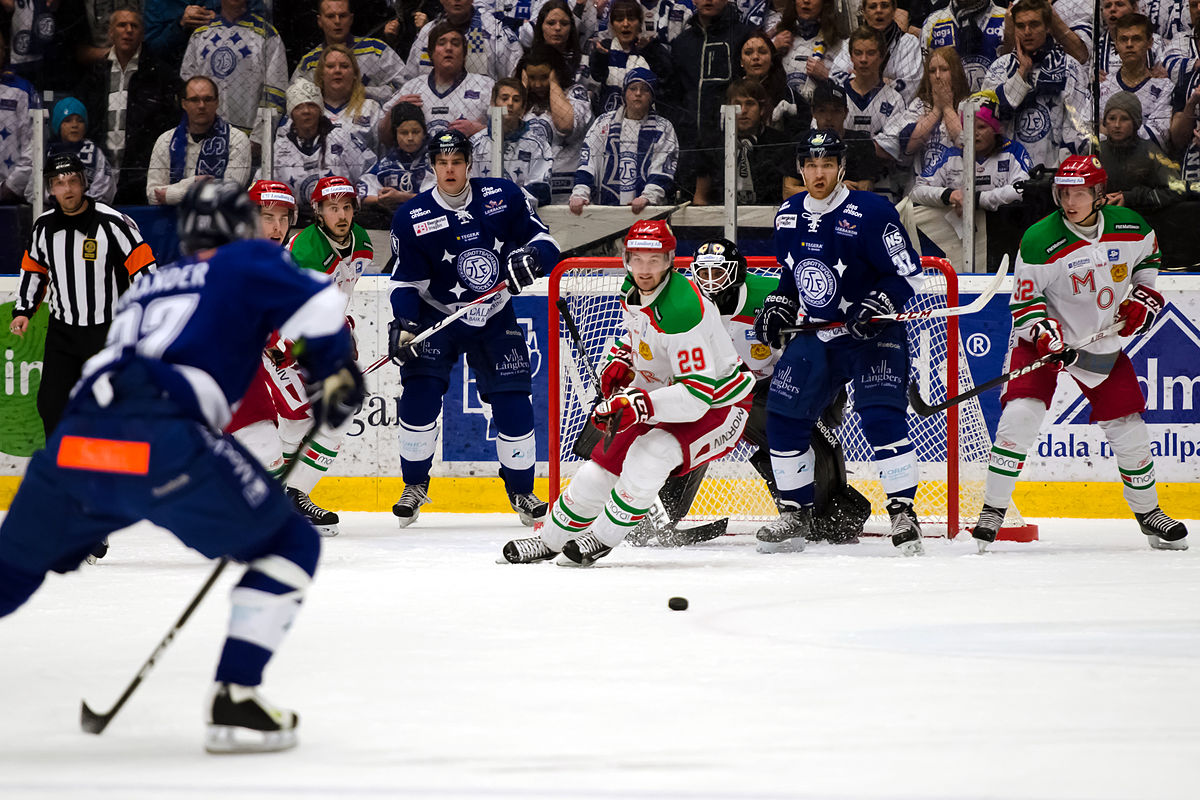
\includegraphics[width=0.6\textwidth]{fig/2012-12-29_skott_01.jpg}
        \begin{imcredit}{90mm}{85mm}
           Image by Calle Eklund \\ Wikimedia Commons
        \end{imcredit}
	\caption{A hockey game. \label{fig:4_hockey}}
\end{figure}

There is a substantial body of research into modeling goal scoring in hockey.
One tactical problem that has been carefully studied is the question of when the goalie should be pulled -- that is, when a team is down by one goal (or more) in the late game, their coach must decide when the right time is to replace the goalie with another attacking skater.
Modeling the game allows analyses to be performed in different scenarios.
In \cite{t07} and \cite{bs10}, for example, a hockey game is modeled as a random (Markov) process where interarrival times of goals follow either an exponential or a generalized exponential distribution.
We will not go into as complex a model as these ones; instead we follow \cite{mw86} and try to simulate a more rudimentary model of the game.

When the teams are of equal quality, we assume that while both teams have all six players on the ice (the goalie and five attackers), 
they are of equal ability, and each team scores goals independently at a rate of $\lambda$ per minute.  
This is the simplest framework that we can assume for modeling a hockey game; let us try to model it in Excel.

To simulate one period of a hockey game, for each team we generate a sequence of exponentially-distributed random variables, and stop once the sum of the generated values exceeds 20 minutes.
For instance, using $\lambda = 0.1$ goals/min and the inverse function technique from Section~\ref{sec:2_expo}, we obtain the following interarrival times: 5.88, 12.13, 13.22, 2.43, $\ldots$.
This means that goals were scored by that team at 5.88 and 18.01 minutes, for a total of two goals in the first period (since the sum of the first three values already exceeds 20).

We repeat the same process for the other team, and for the second and third periods (resetting when each period starts).
Here's what it looks like in Excel:

\begin{figure}[htbp]
	\centering
	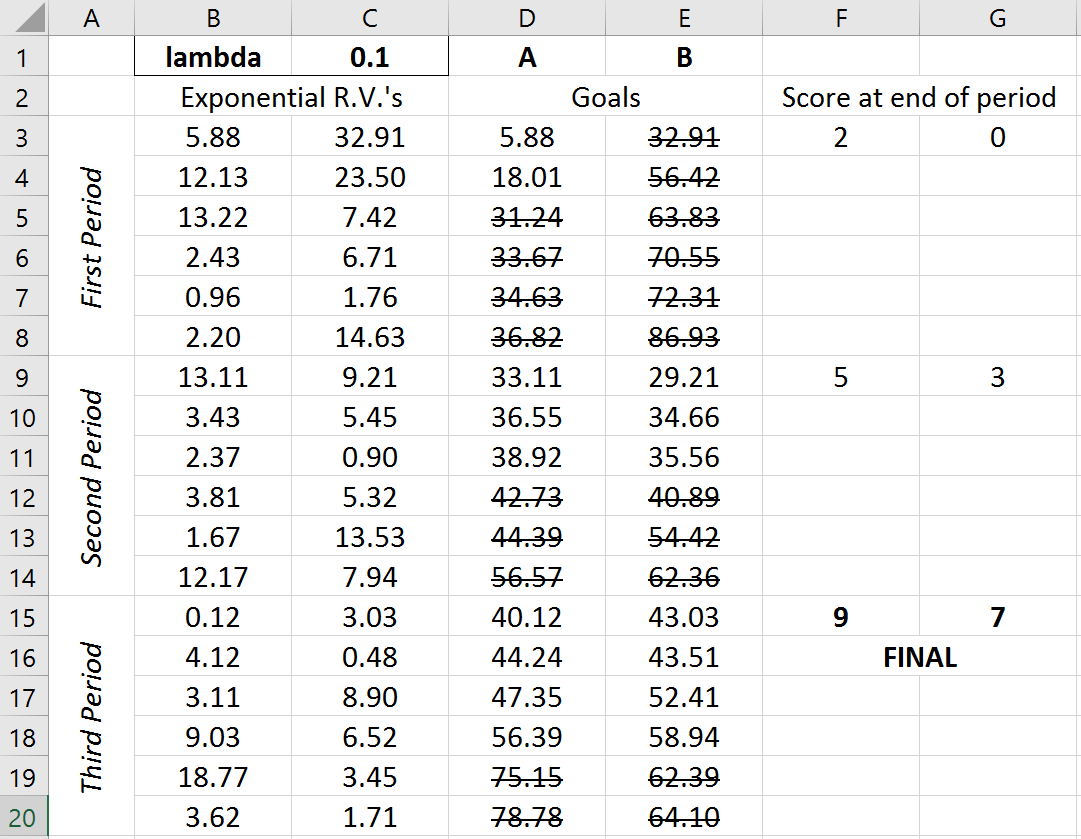
\includegraphics[width=0.6\textwidth]{fig/4_hockey1.png}
	\caption{Simulating a hockey game. \label{fig:4_hockey1}}
\end{figure}

The corresponding formulas are as follows:

\begin{figure}[htbp]
	\centering
	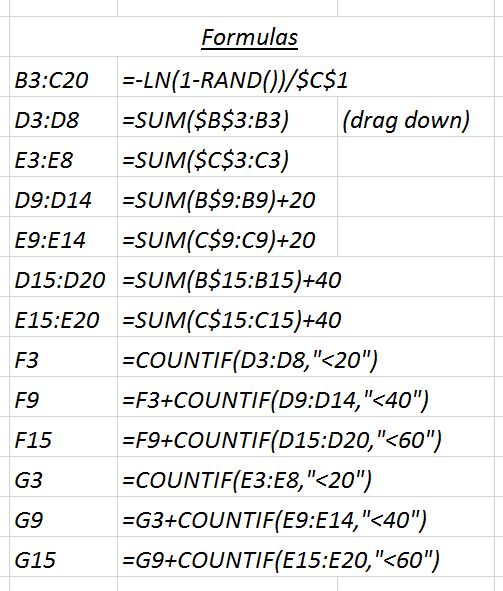
\includegraphics[width=0.3\textwidth]{fig/4_hockeyformulas.png}
	\caption{Formulas for the Excel spreadsheet in Figure~\ref{fig:4_hockey1}. \label{fig:4_hockeyformulas}}
\end{figure}

Observe that to get times in the second and third periods (columns \texttt{C} and \texttt{D}), we added 20 and 40 (respectively) to the same formula we used in the first period.
Furthermore, these cells have been formatted such that values that are above the possible period times are struck-through.
Finally, the \texttt{COUNTIF} function outputs the actual number of goals at the end of each period.

Indeed, the scoring rate $\lambda$ for the two teams can be different, and it is an easy change in the spreadsheet to adopt this.
Nevertheless, it is an entirely different problem to estimate $\lambda$ for actual teams -- for this one needs to go into data fitting and parameter estimation, which are beyond the focus of this Chapter.
What we are interested in is running the simulation \emph{given} the $\lambda$ values.

A few more observations:
\begin{itemize}
	\item The Excel spreadsheet we used only generated six exponential random variables in each period, for each team.
		This might not be enough if $\lambda$ is increased; if $\lambda = 0.4$ goals/min, for example, this translates into a rate of 8 goals per 20-minute period.
		While not necessarily realistic, the model should generate enough random variates such that the sum of the interarrival times is larger than 20.
		This is one limitation of Excel, in that we need to specify in advance how many we are generating.
	\item Penalties and power plays are not considered in the above simulation; a complete model would take into account different `states': 5 vs.~5, 5 vs.~4, etc, and have different values of $\lambda$ for each team, for each of these cases.
	\item A team can have different values of $\lambda$ depending on the \emph{individual players} on the ice.
		This will be extremely difficult to model, though.
	\item Simulating goalie-pulling is a bit more involved; generally, a team will only pull their goalie when it is late in the third period, and they are only one or two points behind.
		One also needs to run simulations for different scenarios: pulling the goalie with a minute left, with 2 minutes left, etc.
\end{itemize}

\begin{figure}[htbp]
	\centering
	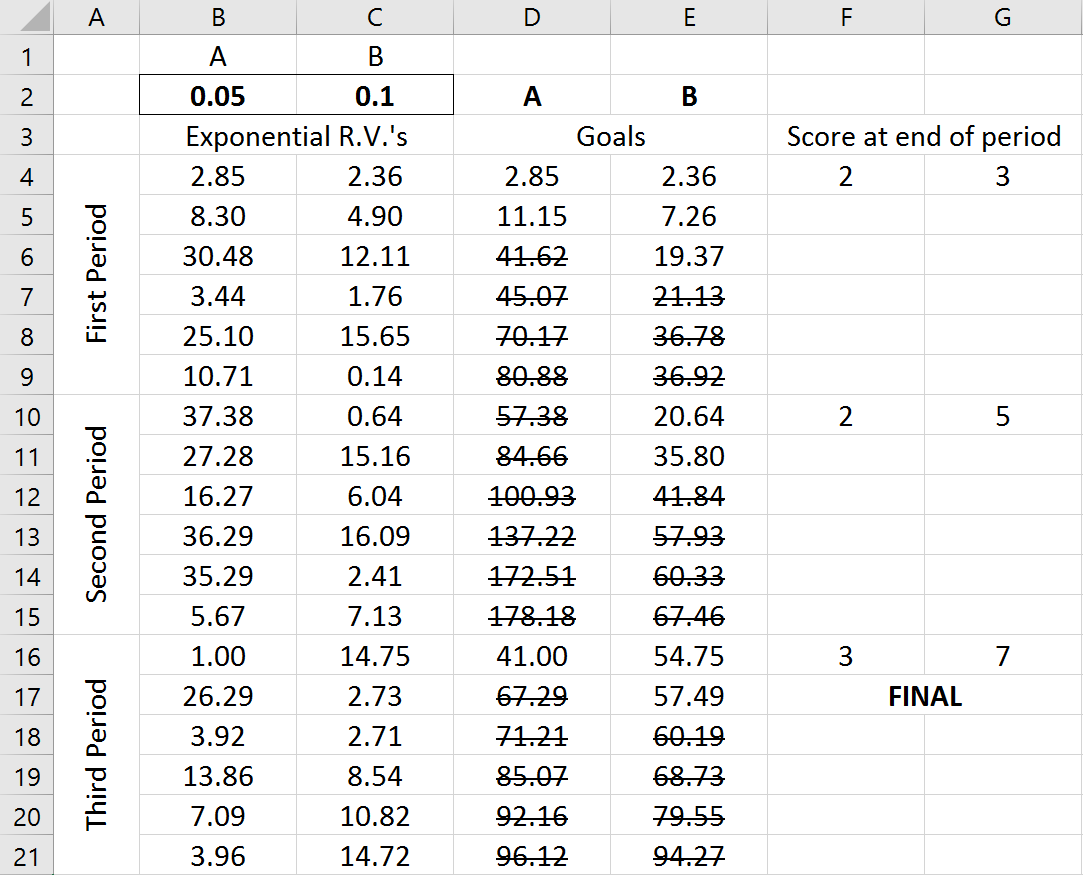
\includegraphics[width=0.6\textwidth]{fig/4_hockey2.png}
	\caption{Simulating a hockey game where the two teams have different scoring rates. \label{fig:4_hockey2}}
\end{figure}


\newpage
\begin{center}
	\textbf{EXERCISES}
\end{center}

\begin{enumerate}[label={4.\arabic*},leftmargin=1cm]
	\item Simulate an M/M/1 queue in excel with $\lambda = 3$/hour and $\mu = 6$/hour until 20 customers are served.
		Compute the average waiting time and average time in the system for customers.
		Then compute the proportion of time that the server is idle.
	\item Simulate an M/M/1 queue in excel with $\lambda = 6$/hour and $\mu = 3$/hour until 20 customers are served.
		Compute the average waiting time and average time in the system for customers.
		Then compute the proportion of time that the server is idle.
		
		Use the technique in Example~\ref{ex:4_MM1} to produce a graph of the simulation you produced.
		In theory, since customers are arriving faster than they can be served, the length of the queue will blow up as time goes to infinity.
		Does your graph confirm this?
	\item Simulate an M/M/2 queue in Excel with $\lambda = 8$/hour and $\mu = 5$/hour until 20 customers are served. \label{ex:4_MM2}
		Compute the average waiting time for customers, then compute the proportion of time that the server is idle.
	\item Compare the M/M/2 queue in Exercise~\ref{ex:4_MM2} with an M/M/1 queue where $\lambda = 8$/hour and $\mu = 10$/hour.
		Do you think the expected waiting times will be similar?
		Simulate this queue and compare.

		How about \underline{two} M/M/1 queues with $\lambda = 4$/hour and $\mu = 5$/hour -- can this be compared to the single M/M/2 queue in Exercise~\ref{ex:4_MM2}?
		Explain what assumptions might have to be made.
	\item In the M/D/1 model, the `D' stands for degenerate, meaning service times are constant.
		This is sometimes a reasonable assumption to make; it comes up in systems where the service requires the same tasks for each customer.
		Let the service time be $\mu$.
		Create a spreadsheet in Excel to model this queue for varying values of $\lambda$ and $\mu$.
	\item Simulate an M/G/1 queue where the service times are normally distributed $\sim N(\mu,\sigma)$.
		For fixed $\lambda$ and $\mu$, what effect do you think changing $\sigma$ has on the average waiting time of a customer?
		Use Excel to study the behaviour of the queue.
		(Hint: What happens as $\sigma \rightarrow 0$?)
	\item \textbf{Critique}. Is it reasonable to assume that interarrival times between goals in a hockey game are exponentially-distributed?
		Why or why not?
	\item Simulate a number of hockey games between two teams where $\lambda = 0.07$ for both.
		Mathematically, excluding ties, each team should win over the other half of the time.
		Does your experiment confirm this?
	\item \textbf{Overtime}. Adapt the spreadsheet in Figure~\ref{fig:4_hockey2} to include an overtime scenario when the score is tied after regulation play.
		Is it reasonable to assume that a 3-on-3 manpower situation will have the same $\lambda$ values as 5-on-5?
	\item \textbf{Pulling the goalie}. Simulate a few hockey games where the goalie is pulled by the team that is trailing with \underline{one minute} left in regulation play.
		Make assumptions on the $\lambda$ parameters for the two teams, and justify your choices.
\end{enumerate}

